\documentclass[aspectratio=169,11pt]{beamer}

\usepackage[T1]{fontenc}
\usepackage[utf8]{inputenc}
\usepackage[french]{babel}
\usepackage{lmodern}
\usepackage{booktabs}
\usepackage{tabularx}
\usepackage{graphicx}
\graphicspath{{../images/}{../../bases/fpga/figures/}}
\usepackage{listings}
\usepackage{tikz}
\usetikzlibrary{positioning,arrows.meta,fit,shapes.geometric,babel}

\usetheme[progressbar=frametitle,numbering=fraction]{metropolis}
\setbeamertemplate{footline}[text line]{\hfill\insertframenumber/\inserttotalframenumber}
\setbeamerfont{footline}{size=\tiny}

\definecolor{acc}{RGB}{235,129,27}
\definecolor{blu}{RGB}{0,95,115}
\definecolor{codebg}{gray}{0.95}
\newcommand{\cmd}[1]{\texttt{\textcolor{blu}{#1}}}
\newcolumntype{L}{>{\raggedright\arraybackslash}X}

\lstset{
  basicstyle=\ttfamily\scriptsize,
  backgroundcolor=\color{codebg},
  frame=none, columns=fullflexible, keepspaces=true,
  breaklines=true, showstringspaces=false,
  commentstyle=\color{gray}, morecomment=[l]{\#},
  literate={é}{{\'e}}1 {è}{{\`e}}1 {à}{{\`a}}1 {ê}{{\^e}}1 {É}{{\'E}}1 {ç}{{\c c}}1
           {«}{{\guillemotleft}}1 {»}{{\guillemotright}}1 {…}{{\ldots}}1 {→}{{$\rightarrow$}}1
           {✓}{{$\checkmark$}}1 {✗}{{$\times$}}1
}

\tikzset{
  box/.style={draw=blu, fill=blu!8, rounded corners=3pt, align=center,
              font=\scriptsize, minimum height=8mm, inner sep=3pt},
  llm/.style={box, draw=acc, fill=acc!12},
  arr/.style={-{Stealth[length=2mm]}, thick, gray!70!black},
  lbl/.style={font=\tiny\itshape, text=gray!40!black},
  layer/.style={draw=blu, fill=blu!#1, minimum height=8mm, align=left,
                font=\scriptsize, anchor=west, inner xsep=6pt}
}

\title{PaperDatabase}
\subtitle{Une base de connaissance textuelle et vérifiable\\pour la lecture assistée d'articles scientifiques}
\author{Léonard Rivals \and Maksym Lytvynenko}
\date{Octobre 2026}

\begin{document}

\maketitle

% ---------------------------------------------------------------------------
\begin{frame}{Le problème}
  Préparer une thèse = lire, comparer et citer des \alert{dizaines d'articles}.
  Un LLM peut aider, mais sur des PDF bruts il travaille mal :
  \vspace{0.6em}
  \begin{itemize}
    \item il \alert{relit le texte intégral} à chaque question (coût, contexte perdu) ;
    \item il \alert{ne sait pas où chercher} un chiffre (tableau ? figure ? annexe ?) ;
    \item il \alert{mélange} ce que dit l'article et ce qu'il en déduit ;
    \item il peut \alert{inventer} une référence ou une valeur plausible.
  \end{itemize}
  \vspace{0.6em}
  \begin{block}{Objectif}
    Des réponses \textbf{sourcées et vérifiables}, à faible coût en tokens, sur n'importe quel corpus.
  \end{block}
\end{frame}

% ---------------------------------------------------------------------------
\begin{frame}{L'idée}
  \begin{columns}[T]
    \begin{column}{0.55\textwidth}
      Convertir chaque PDF en \textbf{fichiers texte structurés} :
      \begin{itemize}
        \item métadonnées vérifiées, sections numérotées et paginées ;
        \item références extraites ;
        \item fiche de lecture et chiffres rangés dans un CSV.
      \end{itemize}
      \medskip
      Le LLM (Claude Code) lit la \alert{couche la plus haute} qui répond,
      et ne descend que si nécessaire.
    \end{column}
    \begin{column}{0.42\textwidth}
      \begin{exampleblock}{Pas de base de données}
        La source de vérité est une arborescence de fichiers texte :
        \textbf{lisible, greppable, diffable, réparable à la main}.
      \end{exampleblock}
      \begin{block}{Par-dessus}
        Un index de passages local (BM25 + embeddings), \textbf{régénérable},
        qui ne modifie aucun fichier.
      \end{block}
    \end{column}
  \end{columns}
\end{frame}

% ---------------------------------------------------------------------------
\begin{frame}{Vue d'ensemble}
  \centering
  \begin{tikzpicture}[node distance=5mm and 8mm, scale=1.12, every node/.append style={transform shape}]
    \node[box] (src) {arXiv id\\DOI\\PDF local};
    \node[box, right=of src] (pap) {\texttt{papers/<id>/}\\métadonnées, texte,\\sections, refs};
    \node[llm, right=of pap] (fic) {\texttt{fiche.md}\\+ lignes de\\\texttt{benchmarks.csv}};
    \node[box, right=of fic] (idx) {\texttt{INDEX.md}\\\texttt{external\_refs.csv}\\index de passages};
    \node[llm, below=12mm of idx] (q) {Questions\\sourcées};
    \node[llm, below=12mm of fic] (gap) {\texttt{gaps.md}};
    \node[box, below=12mm of pap] (disc) {Candidats\\(OpenAlex)};

    \draw[arr] (src) -- node[lbl, above]{\cmd{pdb add}} (pap);
    \draw[arr] (pap) -- node[lbl, above]{\cmd{/paper-fiche}} (fic);
    \draw[arr] (fic) -- node[lbl, above]{\cmd{reindex}} (idx);
    \draw[arr] (idx) -- node[lbl, right]{\cmd{/paper-ask}} (q);
    \draw[arr] (fic) -- node[lbl, right]{\cmd{/paper-gaps}} (gap);
    \draw[arr] (gap) -- (disc);
    \draw[arr] (disc) -| node[lbl, pos=0.25, below]{\cmd{/paper-discover}} (src);
  \end{tikzpicture}

  \vspace{0.8em}
  {\scriptsize
  \tikz\node[box, minimum height=3mm]{}; scripts déterministes (\cmd{bin/pdb})\qquad
  \tikz\node[llm, minimum height=3mm]{}; travail de Claude Code (skills \cmd{/paper-…})}
\end{frame}

% ---------------------------------------------------------------------------
\begin{frame}{Qui fait quoi}
  \renewcommand{\arraystretch}{1.5}
  \begin{tabularx}{\textwidth}{@{}lL@{}}
    \toprule
    \textbf{Qui} & \textbf{Fait quoi} \\
    \midrule
    \textbf{Vous} & choisir les articles, déposer les PDF sous paywall, valider les ajouts
                    et les changements de profil, relire une fiche contre le PDF \\
    \textbf{Les scripts} (\cmd{bin/pdb}) & télécharger, extraire (GROBID), indexer, vérifier
                    la cohérence, chercher des candidats --- \alert{sans LLM} \\
    \textbf{Claude} (\cmd{/paper-…}) & lire, ficher, chiffrer, comparer, relever les gaps,
                    trier les candidats --- \alert{toujours en citant sa source} \\
    \bottomrule
  \end{tabularx}
\end{frame}

% ---------------------------------------------------------------------------
\section{Comment ça marche}

\begin{frame}{1. Acquisition et extraction}
  \begin{columns}[T]
    \begin{column}{0.48\textwidth}
      \textbf{\cmd{bin/pdb add}}
      \begin{itemize}
        \item arXiv : API + PDF ;
        \item DOI : version arXiv trouvée via \textbf{OpenAlex} ;
        \item PDF local, avec export \texttt{.bib}/\texttt{.ris} éditeur ;
        \item lots : \cmd{-{}-from liste.txt}.
      \end{itemize}
      \medskip
      {\small Aucun contournement de paywall : ces PDF se déposent à la main dans \texttt{inbox/}.}
    \end{column}
    \begin{column}{0.48\textwidth}
      \textbf{\cmd{ingest} : GROBID (Docker)}
      \begin{itemize}
        \item fusion des métadonnées (\texttt{.bib} > arXiv > GROBID ; inconnu = \texttt{null}) ;
        \item nettoyage : en-têtes, n\textsuperscript{os} de page, ligatures perdues ;
        \item tableaux : PyMuPDF, puis Docling (+ OCR), marqués « à vérifier » ;
        \item repli PyMuPDF si GROBID est absent ;
        \item idempotent ; \cmd{-{}-reparse} sans GROBID.
      \end{itemize}
    \end{column}
  \end{columns}
\end{frame}

% ---------------------------------------------------------------------------
\begin{frame}{2. Un article = un dossier}
  \small
  \renewcommand{\arraystretch}{1.25}
  \begin{tabularx}{\textwidth}{@{}lL@{}}
    \toprule
    \textbf{Fichier} & \textbf{Contenu} \\
    \midrule
    \texttt{metadata.json}  & titre, auteurs, année, venue, DOI/arXiv, preprint signalé, axes, tags, statut \\
    \texttt{fulltext.md}    & texte intégral nettoyé, sections avec leur numérotation d'origine \\
    \texttt{sections.jsonl} & une ligne par section : type (abstract, section, figure, table) et \alert{page} \\
    \texttt{refs.jsonl}     & références citées : titre, auteurs, année, DOI, arXiv id \\
    \texttt{fiche.md}       & \textcolor{acc}{fiche de lecture} : problème, méthode, résultats, limites, pertinence, lu vs déduit \\
    \texttt{claims.jsonl}   & \textcolor{acc}{preuves atomiques} : une affirmation par ligne, liée à un passage vérifié \\
    \texttt{paper.pdf}      & la preuve d'origine (non versionnée) \\
    \bottomrule
  \end{tabularx}

  \medskip
  Identifiant stable : \texttt{arxiv-2507.18174-real-time-object-detection-classification}
\end{frame}

% ---------------------------------------------------------------------------
\begin{frame}{3. Lire du résumé vers le détail}
  \centering
  \begin{tikzpicture}
    \node[layer=30, minimum width=40mm] (l1) at (0,0)      {\textbf{1} \texttt{INDEX.md}};
    \node[layer=24, minimum width=55mm] (l2) at (0,-0.95)  {\textbf{2} \texttt{benchmarks.csv}};
    \node[layer=18, minimum width=70mm] (l3) at (0,-1.9)   {\textbf{3} \texttt{papers/<id>/fiche.md}};
    \node[layer=12, minimum width=85mm] (l4) at (0,-2.85)  {\textbf{4} passages : \cmd{search} \(\to\) \cmd{show} \(\to\) \cmd{verify}};
    \node[layer=5,  minimum width=100mm, dashed] (l5) at (0,-3.8) {\phantom{\textbf{4}} \texttt{fulltext.md} \quad\textit{(dernier recours)}};

    \node[lbl, font=\scriptsize\itshape, right=3mm of l1.east, anchor=west] {quels articles existent, par axe};
    \node[lbl, font=\scriptsize\itshape, right=3mm of l2.east, anchor=west] {tous les chiffres, 1 ligne = 1 configuration};
    \node[lbl, font=\scriptsize\itshape, right=3mm of l3.east, anchor=west] {l'analyse critique d'un article};
    \node[lbl, font=\scriptsize\itshape, right=3mm of l4.east, anchor=west] {2--3 passages exacts, citations contrôlées};
    \node[lbl, font=\scriptsize\itshape, right=3mm of l5.east, anchor=west] {texte intégral};

    \draw[arr, acc, line width=1.5pt] (-0.5,0.2) -- node[lbl, rotate=90, above]{coût en tokens} (-0.5,-4.0);
  \end{tikzpicture}

  \vspace{0.4em}
  {\small À côté : \texttt{gaps.md} (zones non couvertes, chacune appuyée par des \texttt{paper\_id}),
  \texttt{external\_refs.csv} (travaux absents les plus cités).}
\end{frame}

% ---------------------------------------------------------------------------
\begin{frame}{4. Recherche de passages (style RAG, sans génération)}
  \begin{columns}[c]
    \begin{column}{0.46\textwidth}
      \centering
      \begin{tikzpicture}[node distance=4mm and 4mm]
        \node[box] (q) {question};
        \node[box, below left=of q, xshift=6mm] (b) {BM25\\(lexical)};
        \node[box, below right=of q, xshift=-6mm] (e) {bge-small\\(dense)};
        \node[box, below=16mm of q] (r) {fusion RRF};
        \node[box, below=of r, dashed] (rr) {rerank (option)};
        \node[llm, below=of rr] (o) {passages + \texttt{chunk\_id}, section, page};
        \draw[arr] (q) -- (b); \draw[arr] (q) -- (e);
        \draw[arr] (b) -- (r); \draw[arr] (e) -- (r);
        \draw[arr] (r) -- (rr); \draw[arr] (rr) -- (o);
      \end{tikzpicture}
    \end{column}
    \begin{column}{0.52\textwidth}
      \begin{itemize}
        \item \cmd{search} : passages classés, \alert{rien n'est généré} ;
        \item \cmd{show <chunk\_id>} : texte exact du passage ;
        \item \cmd{verify <chunk\_id> "…"} : la citation y figure-t-elle, \alert{nombres compris} ?
        \item \cmd{bench}, \cmd{paper}, \cmd{cites}, \cmd{compare} : requêtes sans LLM.
      \end{itemize}
      \medskip
      {\small Essai réel : \textbf{$\sim$2\,500 tokens} lus au lieu des textes intégraux.\\
      Route GPU optionnelle : Qwen3-Embedding / Reranker-4B, mêmes \texttt{chunk\_id}.}
    \end{column}
  \end{columns}
\end{frame}

% ---------------------------------------------------------------------------
\begin{frame}[fragile]{Exemple : \texttt{pdb search}}
\begin{lstlisting}
$ bin/pdb search "power measurement method on FPGA board" -k 3
chunk             section                   page  snippet
2015-zhang#039.0  Figures et tableaux          9  Figure 14: «Power» «measurement» of on-«board» execution…
2024-zhang#019.2  5.1. Experimental setup     17  …The «FPGA»'s «power» consumption was reported by the
                                                  «power» analyzer of Vivado, as in previous work [9]…
2304.11580#005.2  4.1. Experimental Setup      7  …For the «measurement» of the inference time…
\end{lstlisting}
\vspace{0.3em}
Puis, dans la réponse de \cmd{/paper-ask} :
\begin{lstlisting}
Verdict : partiel
  ✓ méthode de mesure (Vivado power analyzer)          couvert  [2024-zhang#019.2, p. 17]
  ~ puissance carte complète vs. puce                  partiel
  ✗ mesure au wattmètre externe sur plusieurs cartes   absent
\end{lstlisting}
{\scriptsize Sortie de \cmd{search} réelle ; réponse abrégée, à titre d'illustration. Chaque citation est passée par \cmd{verify} avant d'être écrite ; ce qui est déduit est signalé comme tel.}
\end{frame}

% ---------------------------------------------------------------------------
\begin{frame}{5. Principes de fiabilité}
  \begin{columns}[T]
    \begin{column}{0.5\textwidth}
      \begin{itemize}
        \item \textbf{Tout est du texte}, sauf le PDF gardé comme preuve.
        \item \textbf{Chaque chiffre est traçable} : section, tableau ou figure source, \texttt{chunk\_id}.
        \item \textbf{\texttt{n/r}} pour une valeur non rapportée, \alert{jamais d'estimation}.
      \end{itemize}
    \end{column}
    \begin{column}{0.5\textwidth}
      \begin{itemize}
        \item \textbf{Lu vs déduit} : section « Statut de lecture » obligatoire dans chaque fiche.
        \item \textbf{Comparaisons honnêtes} : \cmd{bench -{}-comparable} (même tâche, jeu, split, métrique).
        \item \textbf{Un seul schéma} : \texttt{lib/schema.py}, validé à chaque réindexation.
      \end{itemize}
    \end{column}
  \end{columns}
  \medskip
  \begin{alertblock}{Règle d'or}
    Ne jamais inventer de référence. Un preprint est signalé comme tel ; une valeur \texttt{confidence: low} aussi.
  \end{alertblock}
\end{frame}

% ---------------------------------------------------------------------------
\begin{frame}{6. Les skills Claude Code}
  \small
  \renewcommand{\arraystretch}{1.2}
  \begin{tabularx}{\textwidth}{@{}lL@{}}
    \toprule
    \cmd{/paper-add}      & acquisition, ingestion, réindexation \\
    \cmd{/paper-fiche}    & fiche de lecture + lignes de \texttt{benchmarks.csv}, chaque chiffre avec sa source \\
    \cmd{/paper-extract}  & 10 à 40 preuves atomiques (\texttt{claims.jsonl}), chacune vérifiée \\
    \cmd{/paper-ask}      & réponse sourcée : verdict, checklist couvert / partiel / absent \\
    \cmd{/paper-compare}  & matrice, accords, désaccords, comparaisons impossibles \\
    \cmd{/paper-discover} & candidats (autres bases, puis OpenAlex), ajout après accord \\
    \cmd{/paper-gaps}     & carte des zones non couvertes (\texttt{gaps.md}) \\
    \cmd{/base-profile}   & affine axes et périmètre d'une base --- propose un diff, vous validez \\
    \cmd{/table-review}   & relit les tableaux extraits contre l'image du PDF \\
    \bottomrule
  \end{tabularx}
\end{frame}

% ---------------------------------------------------------------------------
\begin{frame}{7. Faire grandir le corpus}
  \begin{columns}[T]
    \begin{column}{0.55\textwidth}
      \cmd{pdb discover} / \cmd{/paper-discover} :
      \begin{itemize}
        \item \textbf{en arrière} : ce que le corpus cite ;
        \item \textbf{en avant} : ce qui cite le corpus (\cmd{-{}-since 2020}) ;
        \item \textbf{par axe} maigre ou \textbf{par gap} ;
        \item d'abord dans \textbf{mes autres bases}.
      \end{itemize}
      \medskip
      Sortie : \texttt{candidates.csv} avec \texttt{in\_topic}, raisons (« cité par 3 papiers du corpus »), axe probable.
    \end{column}
    \begin{column}{0.42\textwidth}
      \begin{exampleblock}{Mieux vaut 20 fiches solides que 200 PDF non lus}
        Ajouter un papier seulement s'il comble un axe, étaye un gap
        ou complète une lignée. \textbf{Claude n'ajoute rien sans accord.}
      \end{exampleblock}
    \end{column}
  \end{columns}
\end{frame}

% ---------------------------------------------------------------------------
\begin{frame}{8. Plusieurs bases, un seul code}
  \begin{columns}[T]
    \begin{column}{0.45\textwidth}
      Une base = un dossier \texttt{bases/<nom>/} :
      \begin{itemize}
        \item \texttt{base.json} : axes, règles de classement ;
        \item \texttt{profile.md} : thème, périmètre ;
        \item ses papiers, chiffres, gaps, index.
      \end{itemize}
      \smallskip
      {\small\cmd{pdb base new | scan | import}\\
      \cmd{pdb -{}-base drone bench …}}
    \end{column}
    \begin{column}{0.53\textwidth}
      \scriptsize
      \begin{tabular}{@{}lrrr@{}}
        \toprule
        \textbf{Base} & \textbf{Papiers} & \textbf{Fiches} & \textbf{Benchmarks} \\
        \midrule
        \texttt{fpga}      & 104 & 104 & 299 \\
        \texttt{drone}     &  87 &  86 & 352 \\
        \texttt{stage}     &  56 &  56 & 100 \\
        \texttt{yolo-data} &  44 &  44 & 425 \\
        \bottomrule
      \end{tabular}

      \smallskip
      {\tiny Au 18/10/2026. \texttt{fpga} : vision embarquée sur FPGA (thèse) ;
      \texttt{drone} : vision embarquée sur drone ; \texttt{stage} : apprentissage continu sur MCU ;
      \texttt{yolo-data} : préparation des données YOLO.}
    \end{column}
  \end{columns}
  \medskip
  {\small Bases indépendantes (index, caches, candidats propres) ; un article se copie de l'une à l'autre
  sans refaire l'extraction.}
\end{frame}

% ---------------------------------------------------------------------------
\begin{frame}{Visualisation (pour l'humain, pas pour le LLM)}
  \begin{columns}[c]
    \begin{column}{0.66\textwidth}
      \centering
      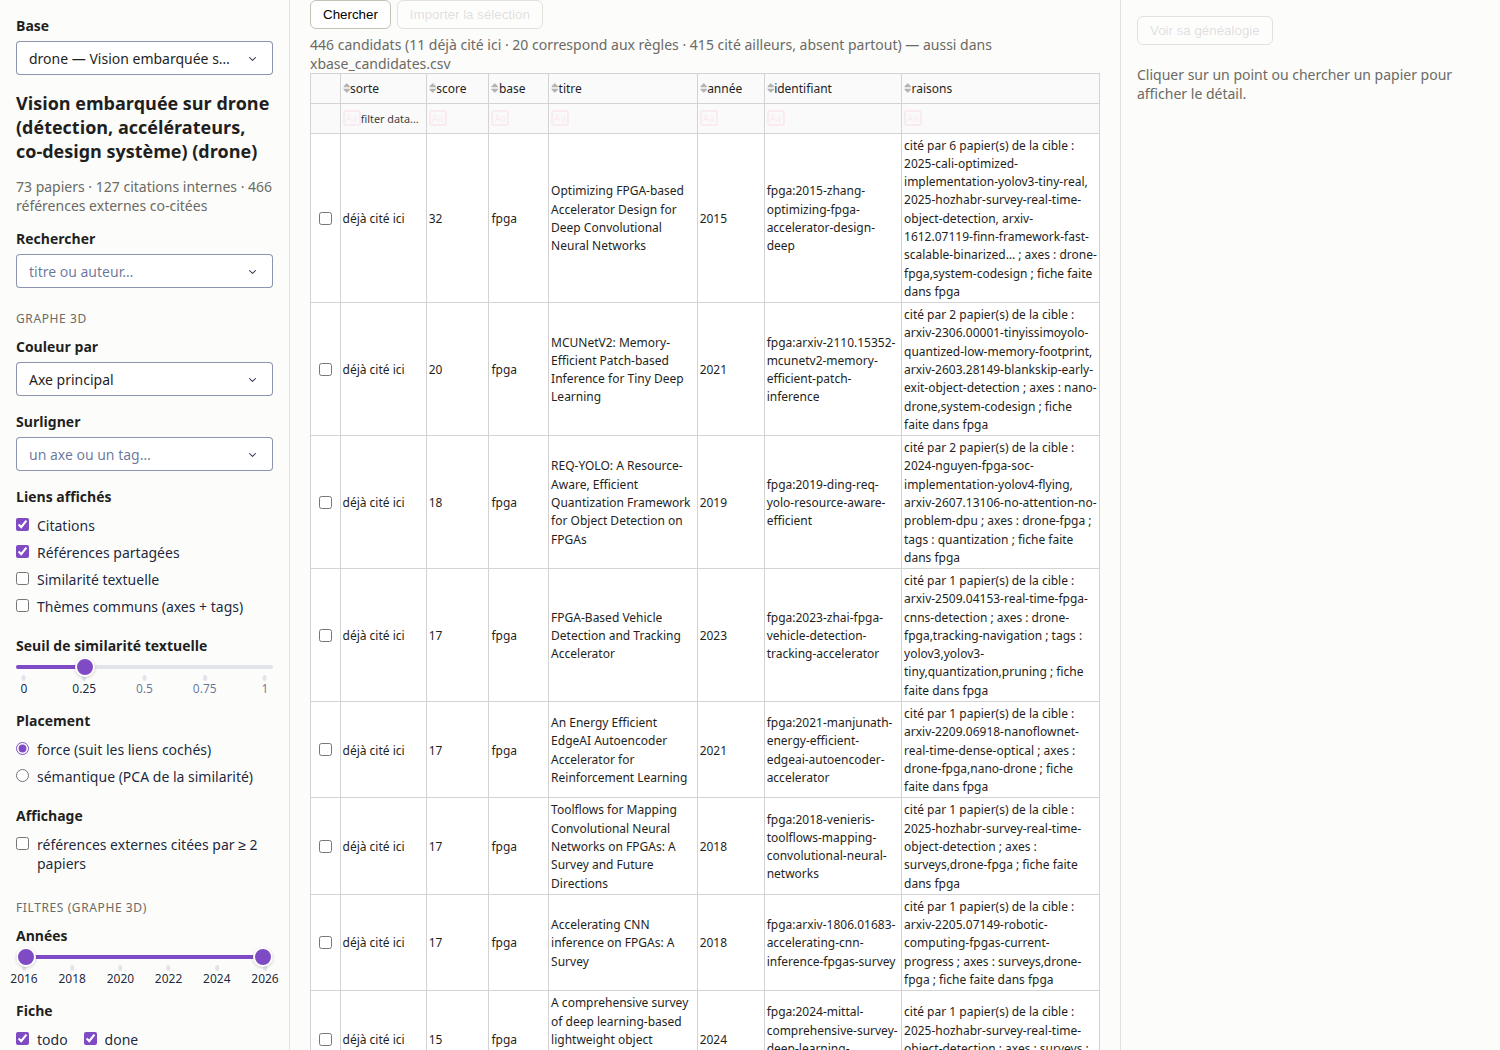
\includegraphics[width=\linewidth,trim=0 620 380 0,clip]{viz-scan.png}\\[2pt]
      {\tiny Onglet Bases : articles de la base \texttt{fpga} déjà cités par la base \texttt{drone}.}
    \end{column}
    \begin{column}{0.32\textwidth}
      \small \cmd{pdb viz} (Dash, local) :
      \begin{itemize}
        \item \textbf{Graphe 3D} : citations, similarité, thèmes ;
        \item \textbf{Généalogie} : frise le long des citations ;
        \item \textbf{Bases} : effectifs, profil, import depuis les autres bases.
      \end{itemize}
      \smallskip
      {\scriptsize N'écrit que sur action explicite (créer une base, importer).}
    \end{column}
  \end{columns}
\end{frame}

% ---------------------------------------------------------------------------
\begin{frame}{Ce que la base produit : exemple \texttt{fpga}}
  \centering
  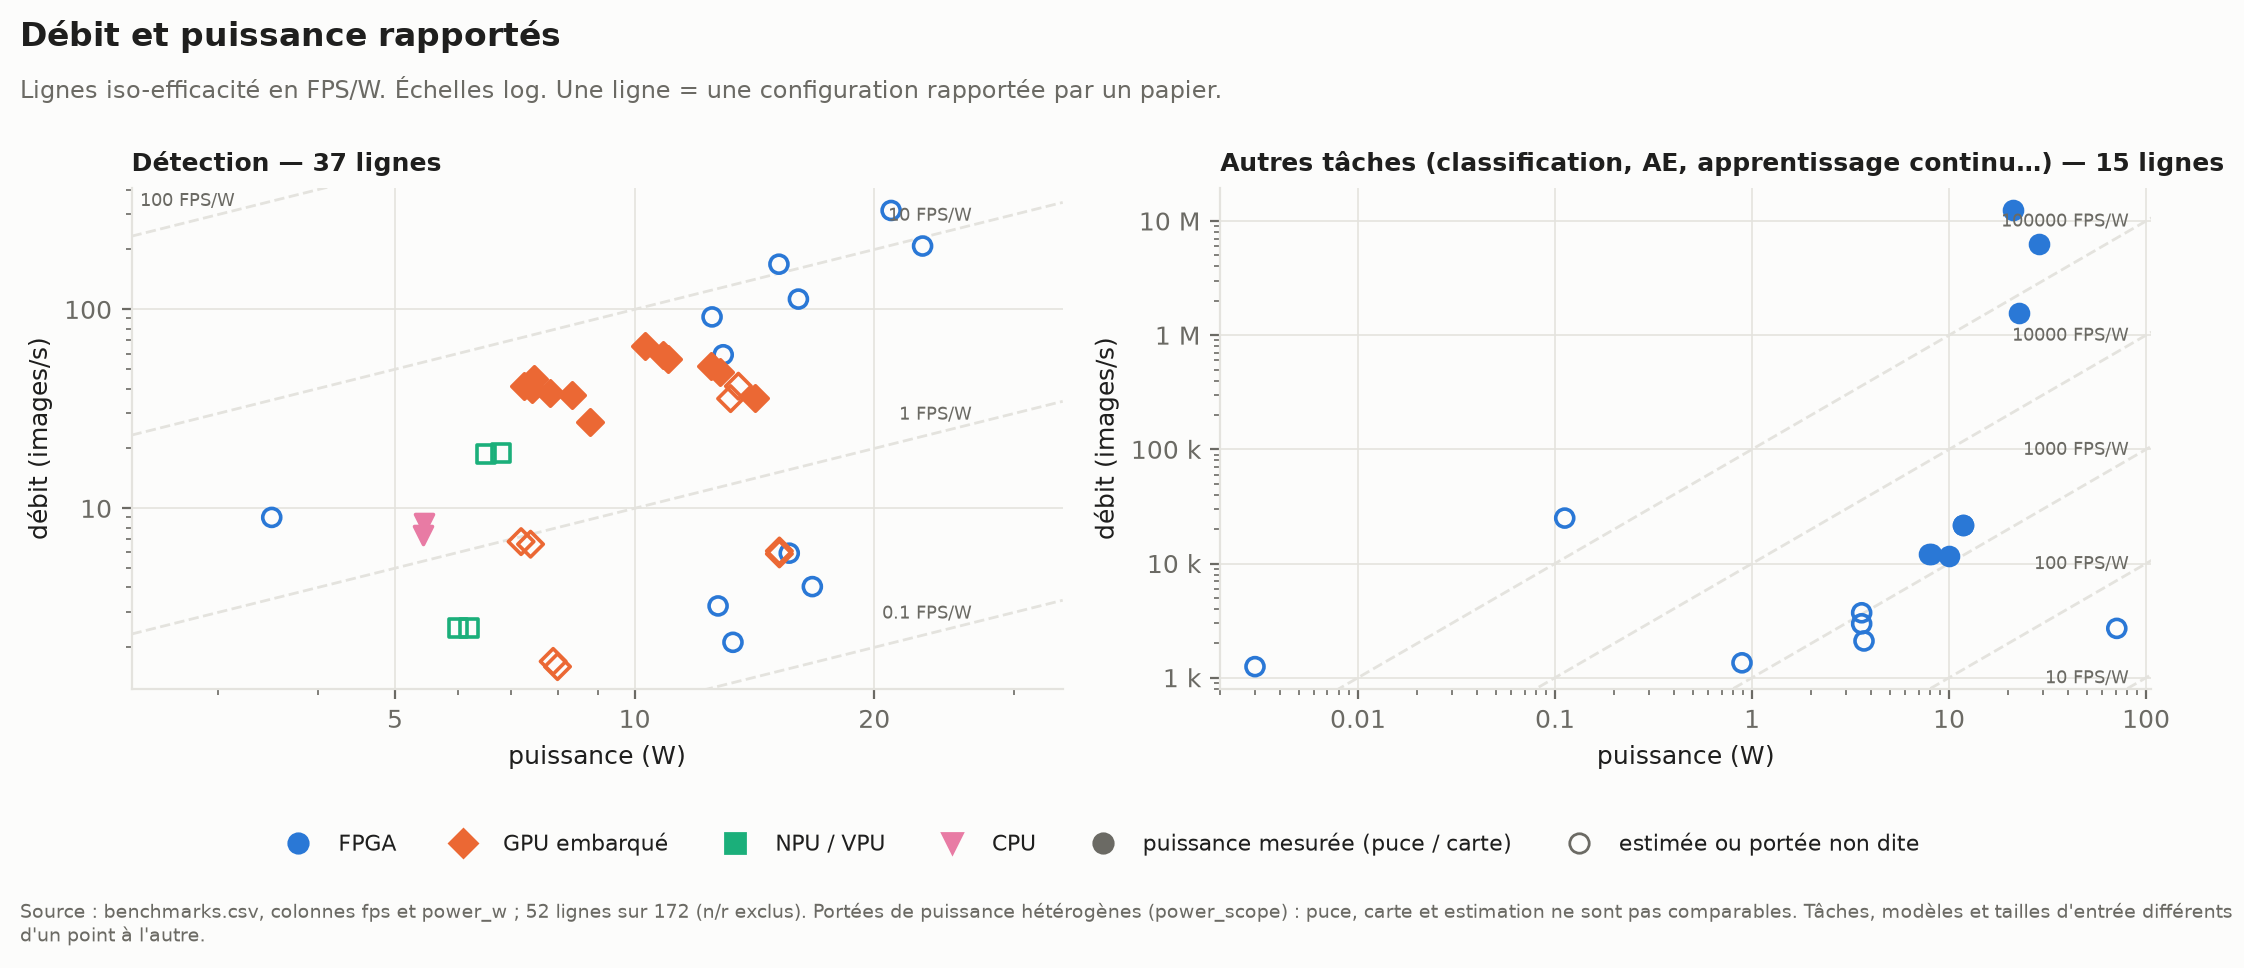
\includegraphics[width=\linewidth,height=0.62\textheight,keepaspectratio]{bench_fps_power.png}

  \small \cmd{pdb plot} trace directement \texttt{benchmarks.csv} (FPS vs puissance, précision vs latence,
  ressources FPGA, GOPS/W, quantification, couverture par axe).
  Chaque point renvoie à un papier et à sa section source.
\end{frame}

% ---------------------------------------------------------------------------
\section{Évaluation et limites}

\begin{frame}{Mesuré par le banc \texttt{pdb eval}}
  \begin{columns}[T]
    \begin{column}{0.32\textwidth}
      \textbf{Recherche} (recall@5)
      \begin{itemize}
        \item \textbf{0,90} anglais, jeu de réglage
        \item \textbf{0,84} jeu jamais vu
        \item \textbf{0,50} en français
      \end{itemize}
    \end{column}
    \begin{column}{0.32\textwidth}
      \textbf{\cmd{verify}}
      \begin{itemize}
        \item \textbf{38/38} citations au chiffre modifié rejetées
        \item \textbf{40/40} citations exactes acceptées
      \end{itemize}
    \end{column}
    \begin{column}{0.32\textwidth}
      \textbf{Extraction}
      \begin{itemize}
        \item \textbf{91\,\%} du texte du PDF retrouvé
        \item \textbf{90\,\%} des tableaux avec leur corps
      \end{itemize}
    \end{column}
  \end{columns}
  \medskip
  \begin{itemize}
    \item Réponses de \cmd{/paper-ask} notées à l'aveugle (\cmd{/eval-answers}) : hors corpus reconnu 6/6,
          verdict juste 0,83 (dev) et 0,92 (holdout).
    \item 288 tests unitaires ; \cmd{pdb eval -{}-compare} avant/après tout changement du pipeline.
  \end{itemize}
\end{frame}

% ---------------------------------------------------------------------------
\begin{frame}{Limites et suite}
  \begin{itemize}
    \item \textbf{Tableaux} : les tableaux reconstruits restent à relire contre le PDF ;
          une valeur de \texttt{benchmarks.csv} n'est retrouvée telle quelle que dans 80\,\% des cas.
    \item \textbf{Absence de sujet} : \cmd{search} renvoie toujours des passages ; aucun score ne dit
          de façon fiable que la base ne traite pas une question.
    \item \textbf{Généricité} : colonnes de \texttt{benchmarks.csv} pensées pour le matériel.
    \item \textbf{Coût} : \cmd{/paper-fiche} lit encore \texttt{fulltext.md} en entier
          (digest déterministe prévu).
    \item \textbf{Traçabilité automatique} : lier chaque ligne de benchmark à un \texttt{chunk\_id} vérifié.
  \end{itemize}
\end{frame}

% ---------------------------------------------------------------------------
\begin{frame}[fragile]{Démarrage rapide}
  Prérequis : Python 3.12, Docker, Claude Code.
\begin{lstlisting}
bash bin/setup.sh                       # .venv + dépendances
bin/pdb grobid start                    # GROBID sur localhost:8070
bin/pdb base new mon-sujet --theme "…"  # une base par sujet
cd bases/mon-sujet && bin/pdb status    # état et prochaines actions
bin/pdb add 2507.18174                  # arXiv id, DOI ou PDF local
\end{lstlisting}
  Puis, dans Claude Code ouvert dans la base :
\begin{lstlisting}
/base-profile                           # axes et périmètre (vous validez)
/paper-fiche <paper_id>                 # fiche + chiffres sourcés
/paper-ask "Quels papiers dépassent 25 FPS sous 5 W ?"
/paper-discover                         # la suite à lire
\end{lstlisting}
  {\small Guide pas à pas : \texttt{docs/GUIDE.md} --- détails : \texttt{SETUP.md}, \texttt{DATA\_MODEL.md}.}
\end{frame}

% ---------------------------------------------------------------------------
\begin{frame}[standout]
  Des PDF \(\to\) du texte structuré \(\to\) des réponses \textbf{sourcées}\\[1em]
  \normalsize Questions ?
\end{frame}

\end{document}
